% !TEX root = SystemTemplate.tex
\chapter{User Stories, Backlog and Requirements}
\section{Overview}


The overview should take the form of an executive summary.  Give the reader a feel 
for the purpose of the document, what is contained in the document, and an idea 
of the purpose for the system or product. 

 The userstories 
are provided by the stakeholders.  You will create he backlogs and the requirements, and document here.  
This chapter should contain 
details about each of the requirements and how the requirements are or will be 
satisfied in the design and implementation of the system.

Below:   list, describe, and define the requirements in this chapter.  
There could be any number of sub-sections to help provide the necessary level of 
detail. 





\subsection{Scope}


What scope does this document cover?  This document would contain stakeholder information, 
initial user stories, requirements, proof of concept results, and various research 
task results. 



\subsection{Purpose of the System}
The purpose of Crowd Control is the ease the user expearence of going out in groups.


\section{ Stakeholder Information}


This section would provide the basic description of all of the stakeholders for 
the project.  Who has an interest in the successful and/or unsuccessful completion 
of this project? 


\subsection{Customer or End User (Product Owner)}
Who?  What role will they play in the project?  Will this person or group manage 
and prioritize the product backlog?  Who will they interact with on the team to 
drive product backlog priorities if not done directly? 

\subsection{Management or Instructor (Scrum Master)}
Who?  What role will they play in the project?  Will the Scrum Master drive the 
Sprint Meetings? 


\subsection{Investors}
Are there any?  Who?  What role will they play? 


\subsection{Developers --Testers}
Who?  Is there a defined project manager, developer, tester, designer, architect, 
etc.? 


\section{Business Need}
Use this section to define what business need exist and how this software will 
meet and/or exceed that business need.   

\section{Requirements and Design Constraints}
Use this section to discuss what requirements exist that deal with meeting the 
business need.  These requirements might equate to design constraints which can 
take the form of system, network, and/or user constraints.  Examples:  Windows 
Server only, iOS only, slow network constraints, or no offline, local storage capabilities. 


\subsection{System  Requirements}
Sense there we are creating Crowd Control to run on two different platforms, both iOS and Android, there are two sets of requirements that will be similar between both platforms. Even though they are both similar, implimentation between both will be differnet. With them both being different they are split into two sections as listed below.

\subsubsection{iOS Requirements}
\begin{itemize}
\item{Use Apple Mapping Features}
\item{Access Parse as the Database}
\end{itemize}
\subsubsection{Android Requirements}
\begin{itemize}
\item{Use Google Maps}
\item{Access Parse as the Database}
\end{itemize}
\subsubsection{Parse Requirements}
\begin{itemize}
\item{Delete groups when group is not in use}
\end{itemize}


\subsection{Network Requirements}
Network requrements are mobile networks as this is a mobile applications. The requirement on our part is making sure that the application is able to reach the server and use at little data as possible when connected to the network. Making sure we use as little data as possible will help our users not use all of their data. 


\subsection{Development Environment Requirements}
The development enviroment requirement is that Crowd Control be avalabe on both iOS and Android platforms. Being cross platform allows for us to reach as many users as possible. Android development will be handled with Android Studio and iOS will be developed with xCode.


\subsection{Project  Management Methodology}
We have set restrictions on the developemnt of Crowd Control and are listed as follows:
 
\begin{itemize}
\item GitHub issues will be used to keep track of current status as well as backlogs for the product.
\item There will be 6 total sprints over 2 scimesters for this products.
\item The sprint cycles are 3 weeks long.
\item Progress reports will be summited to Dr. McGough and Brian Butterfeild at the end of each sprint.
\item Github will be used for source control. 
\end{itemize}

\section{User Stories}
This section can really be seen as the guts of the document.  This section should 
be the result of discussions with the stakeholders with regard to the actual functional 
requirements of the software.  It is the user stories that will be used in the 
work breakdown structure to build tasks to fill the product backlog for implementation 
through the sprints.

This section should contain sub-sections to define and potentially provide a breakdown 
of larger user stories into smaller user stories. 



\subsection{User Story \#1 }
As a user i want to be able to join a group.

\subsubsection{User Story \#1 Breakdown}
As a user i want the ability to join a group. Group joining options would be from a list or from an invite from a user. 

\subsection{User Story \#2} 
As a user i want the abilitiy to track locations of other members in the group.

\subsubsection{User Story \#2 Breakdown}


\subsection{User Story \#3} 
As a user i want post agenda for the group.

\subsection{User Story \#4} 
As a user i want to i want the abilitiy to look for local groups

\subsection{User Story \#5} 
As a user i want the ability to have suggestions of local activities.

\subsection{User Story \#6} 
As a user i want the ability to leave a group.

\subsection{User Story \#7} 
As a user i want the ability to have a list of local groups.

\subsection{User Story \#8} 
As a user i want the abilitiy to login.

\subsection{User Story \#9}
As a user i would like to message other members of the group.

\subsection{User Story \#10} 
As a user i would like my information protected. 

\section{Proof of Concept Results}
The Proof of conecpt is a rough design that impliments basic features of Crowd Control. Basic features are currently under construction. This is currently a functional prototype with improvements in the future.
\newline 
\newline
Below are screen shots of both android and iOS proof of concepts.
(current formatting issues need to fix)
\subsection{iOS Proof of Concept Screen Shots}


	\begin{figure}[tbh]
	\begin{center}
	\includegraphics[width=0.75\textwidth]{iOSPictures/img_3901.png}
	\end{center}
	\caption{iOS login select screen \label{iOSloginselectscreen}}
	\end{figure}

	\begin{figure}[tbh]
	\begin{center}
	\includegraphics[width=0.75\textwidth]{iOSPictures/img_3896.png}
	\end{center}
	\caption{iOS email login screen \label{iOSemailLoginScreen}}
	\end{figure}

	\begin{figure}[tbh]
	\begin{center}
	\includegraphics[width=0.75\textwidth]{iOSPictures/img_3897.png}
	\end{center}
	\caption{iOS create account screen \label{iOScreateAccountScreen}}
	\end{figure}

	\begin{figure}[tbh]
	\begin{center}
	\includegraphics[width=0.75\textwidth]{iOSPictures/img_3898.png}
	\end{center}
	\caption{iOS group infomation screen \label{iOSGroupScreen}}
	\end{figure}

	\begin{figure}[tbh]
	\begin{center}
	\includegraphics[width=0.75\textwidth]{iOSPictures/img_3899.png}
	\end{center}
	\caption{iOS map view screen \label{iOSmapScreen}}
	\end{figure}

	\begin{figure}[tbh]
	\begin{center}
	\includegraphics[width=0.75\textwidth]{iOSPictures/img_3900.png}
	\end{center}
	\caption{iOS messaging main screen \label{iOSmessagingMain}}
	\end{figure}


\subsection{Android  Proof of Concept Screen Shots}

	\begin{figure}[tbh]
	\begin{center}
	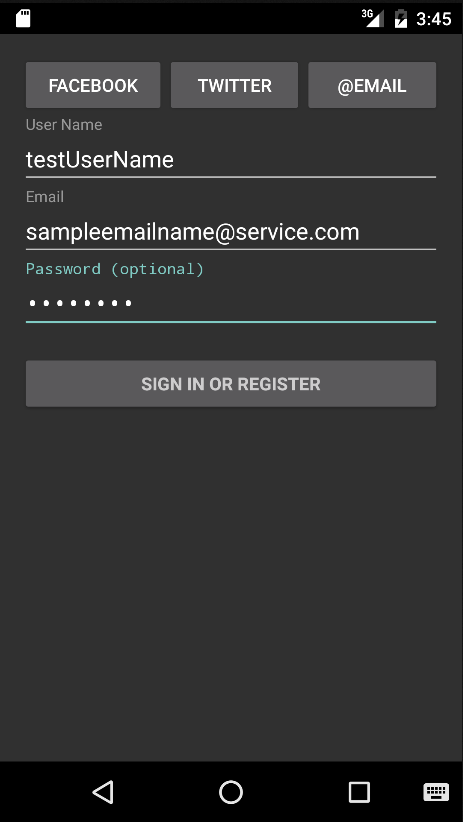
\includegraphics[width=0.75\textwidth]{AndroidPictures/loginScreen.png}
	\end{center}
	\caption{Android login screen \label{AndroudLoginScreen}}
	\end{figure}

	\begin{figure}[tbh]
	\begin{center}
	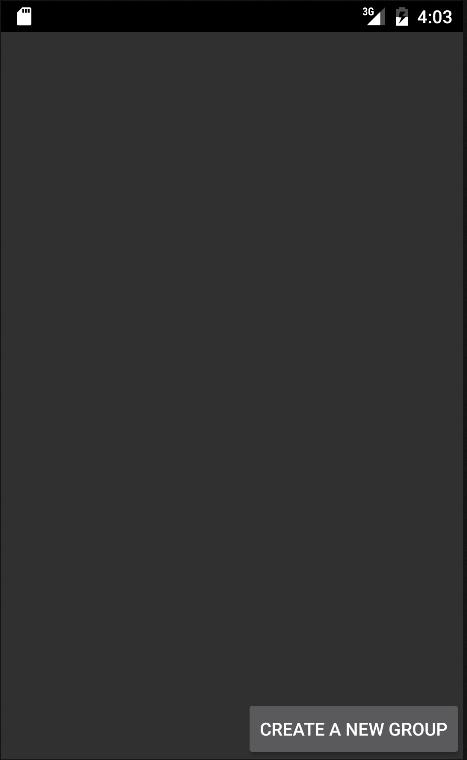
\includegraphics[width=0.75\textwidth]{AndroidPictures/createNewGroup.png}
	\end{center}
	\caption{Android create group screen \label{AndroidCreateGroup}}
	\end{figure}

	\begin{figure}[tbh]
	\begin{center}
	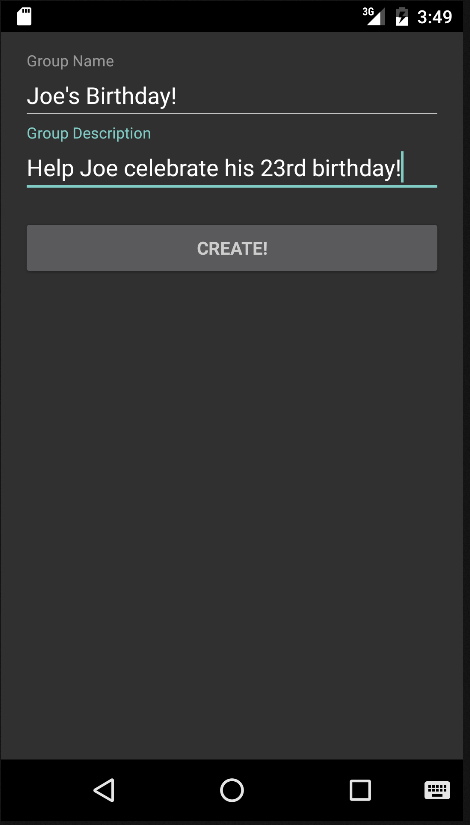
\includegraphics[width=0.75\textwidth]{AndroidPictures/groupCreatePage.png}
	\end{center}
	\caption{Android group information screen \label{AndroidGroupInfo}}
	\end{figure}

	\begin{figure}[tbh]
	\begin{center}
	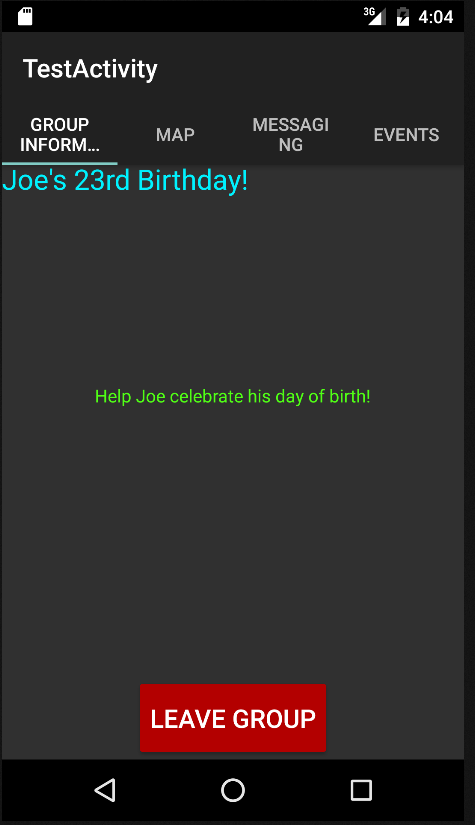
\includegraphics[width=0.75\textwidth]{AndroidPictures/groupJoinedPage.png}
	\end{center}
	\caption{Android group join screen \label{AndroidJoinGroup}}
	\end{figure}

	\begin{figure}[tbh]
	\begin{center}
	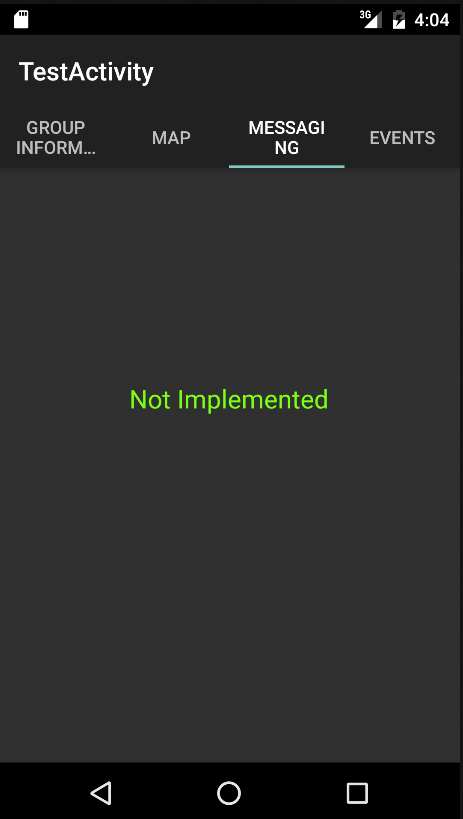
\includegraphics[width=0.75\textwidth]{AndroidPictures/messagingNotImplemented.png}
	\end{center}
	\caption{Android messaging main screen \label{AndroidMessagingMain}}
	\end{figure}


\section{Supporting Material}


This document might contain references or supporting material which should be documented 
and discussed  either here if appropriate or more often in the appendices at the end.  This material may have been provided by the stakeholders  
or it may be material garnered from research tasks.

